\section{Analysis of Variance (ANOVA)}\label{sec:ANOVA}
\textbf{Analysis of variance} (ANOVA) is a statistical method that partitions a dataset's variability into \textbf{explainable variability} (model-based) and \textbf{unexplained variability} (error) using various statistical models, to determine whether (multiple) treatment groups have significantly different group means. 
\newl The \textbf{total sample variability} of a feature $y$ in a dataset is defined as
\begin{equation*}
    \text{SS}_{\textrm{tot}}=\sum_{k=1}^{N}(y_{k}-\bar{y})^{2},
\end{equation*}
where $\bar{y}$ is the overall mean of the data. 
\newl Let us return to the teaching method example given in Section \ref{sec:Hyp.Testing}. \par Figure \ref{fig:testA1} shows all the students' scores, ordered by participant ID. Since the assignment of ID is \textbf{arbitrary} (at least, in theory), we do not observe any patterns -- if we were to guess someone's score with no knowledge except for their participant ID, then picking the sample mean is as good a guess as any other reasonable guesses. \newl Statistically speaking, this means that the \textbf{null model}
\begin{equation*}
    y_{i,j}=\mu+\varepsilon_{i,j},
\end{equation*}
where $\mu$ is the \textbf{overall mean}, $i= {A,B}$, and $j=1,\ldots,40$, does not explain any of the variability in the student scores (as usual, $\varepsilon_{i,j}$ represents the departure or noise from the model prediction).\newl But 
\begin{figure*}[t]
\centering
  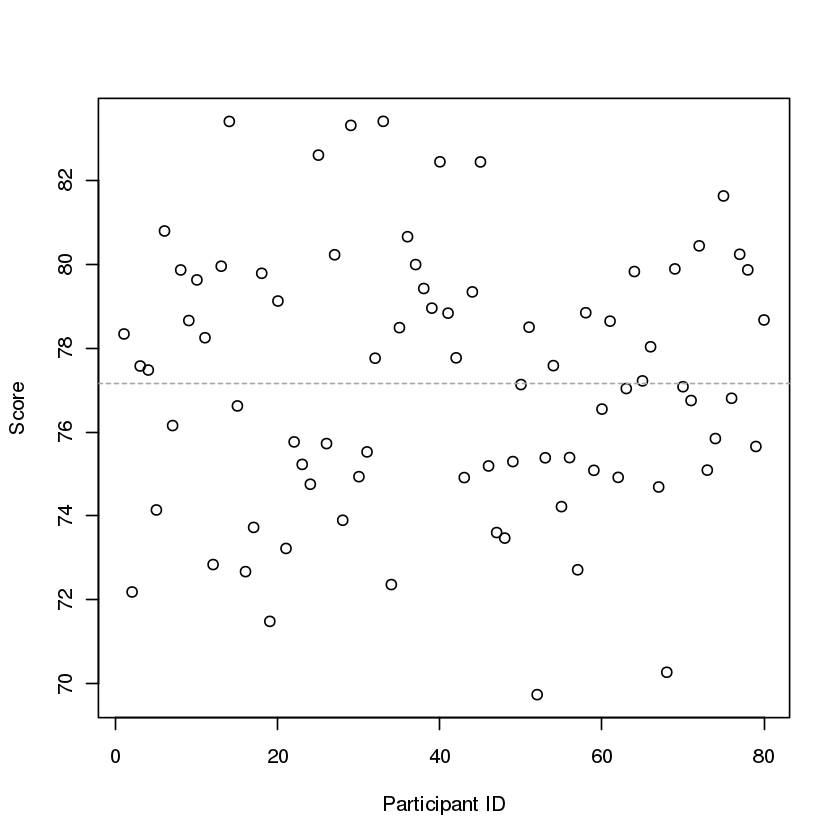
\includegraphics[width=0.485\linewidth]{Images/testA1.png} \quad 
  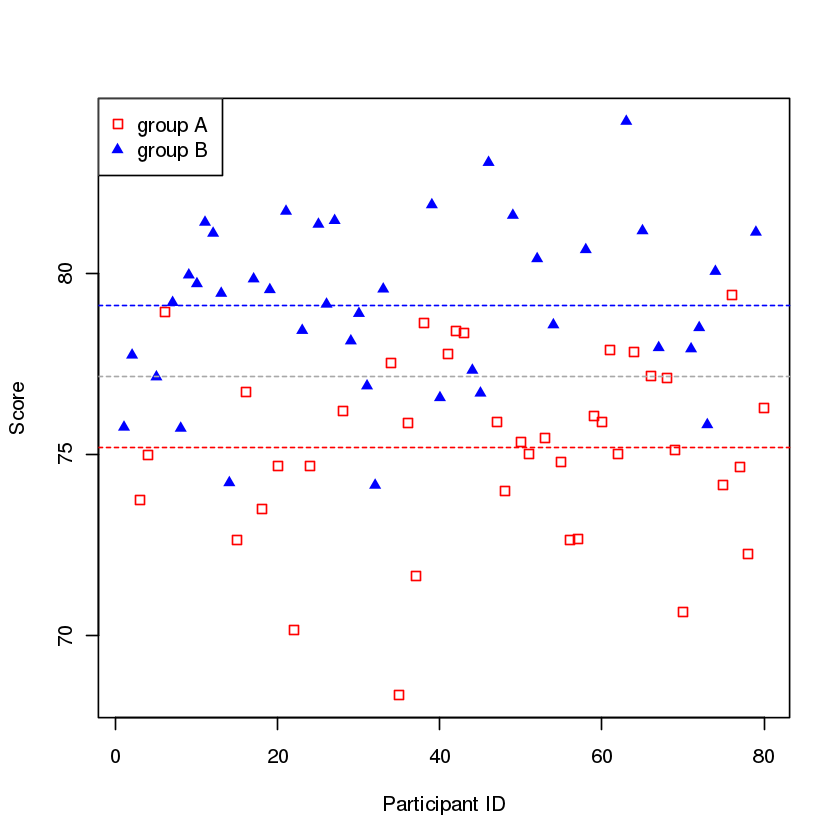
\includegraphics[width=0.485\linewidth]{Images/testA2.png}
  \caption[\small Effectiveness of new teaching method (two groups)]{\small Effectiveness of new teaching method for two groups. The grey line is the overall sample mean (left), while the red and blue lines represent the average score for groups $A$ and $B$, respectively (right).}
  \label{fig:testA1} \hrule
\end{figure*}
the students DID NOT all receive the same treatment: $40$ randomly selected students were assigned to group $A$, and the other $40$ to group $B$, and both group were taught using a different method. \par When we add this information onto Figure \ref{fig:testA1} (on the right), we clearly see that the two study groups show different characteristics in term of their average scores. \newpage\noindent With the group assignment information, we can refine our null model into the  \textbf{treatment-based model}
\begin{equation*}%\label{eq:ANOVA1}
    y_{i,j}=\mu_{i}+\varepsilon_{i,j},
\end{equation*}
where $\mu_i$, $i={A,B}$ represent the group means. \newl Using this model, we can decompose $\text{SS}_{\textrm{tot}}$ into \textbf{between-treatment sum of squares} and \textbf{error (within-treatment) sum of squares} as
\begin{align*}
   \text{SS}_{\textrm{tot}}&=\sum_{i,j}(y_{i,j}-\bar{y})^{2}=\sum_{i,j}(y_{i,j}-\bar{y}_{i}+\bar{y}_{i}-\bar{y})^{2}\\
    &=\sum_{i}N_{i}(\bar{y}_{i}-\bar{y})^{2}+\sum_{i,j}(y_{i,j}-\bar{y}_{i})^2=\text{SS}_{\textrm{treat}}+\text{SS}_{\textrm{e}}
\end{align*}
The $\text{SS}_{\textrm{treat}}$ component looks at the difference between each of the treatment means and the overall mean, which we consider to be \textbf{explainable}\footnote{That is to say, the treatment explains part of the difference in the observed group means.}; the $\text{SS}_{\textrm{e}}$ component, on the other hand, looks at the difference between each observation and its own group mean, and is considered to be \textbf{random}.\footnote{As the spread about the group means is fairly large (relatively-speaking), we suspect that the treatment-based model on its own does not capture all the variability in the data.} 
\par Thus, $\text{SS}_{\textrm{treat}}/\text{SS}_{\textrm{tot}}\times 100\%$ of the total variability can be explained using a treatment-based model. This ratio is called the \textbf{coefficient of determination}, denoted by $R^{2}$.
\newl Formally, the ANOVA table incorporates a few more items -- Table~\ref{tab:SA2} summarises all the information that it contains; the specific table for the teaching methodology example is shown in \ref{tab:SA3}.

     \begin{table*}[t]
         \centering
         \begin{tabular}{c c c c c c}
         \hline
        \textbf{Source} & \textbf{Sum of Squares} & \textbf{df} & \textbf{Mean Square} & $\mathbf{F_{0}}$ & $\mathbf{p-}$\textbf{value}\\
         \hline
         Treatment (Model) & $\text{SS}_{\textrm{treat}}$ & $p-1$ & $\text{MS}_{\textrm{treat}}=\text{SS}_{\textrm{treat}}/(p-1)$ & $\text{MS}_{\textrm{treat}}/\text{MS}_{\textrm{e}}$ & $P(F_0>F^*)$\\
         Error & $\text{SS}_{\textrm{e}}$ & $N-p$ & $\text{MS}_{\textrm{e}}=\text{SS}_{\textrm{e}}/(N-p)$ & \\
         Total & $\text{SS}_{\textrm{tot}}$ & $N-1$ & & \\
        \hline
         \end{tabular}
         \caption[\small A simple ANOVA table]{\small A simple ANOVA table, with $p$ treatments and $N$ observations.}
         \label{tab:SA2}
     \end{table*}


     \begin{table*}[t]
         \centering
         \begin{tabular}{c c c c c c}
         \hline
        \textbf{Source} & \textbf{Sum of Squares} & \textbf{df} & \textbf{Mean Square} & $\mathbf{F_{0}}$ & $\mathbf{p-}$\textbf{value}\\
         \hline
         Treatment (Model) & $300.31$ & $1$ & $300.31$ & $49.28$ & $7.2\times 10^{-10}$ ***\\
         Error & $475.38$ & $78$ & $6.095$ & \\
         Total & $775.69$ & $79$ & & \\
        \hline
         \end{tabular}
         \caption[\small ANOVA table -- teaching methodology]{\small ANOVA table for the teaching methodology example, with $p=2$ and $N=80$, at $\alpha=0.001$.}
         \label{tab:SA3}\hrule
     \end{table*}
The test statistic $F_{0}$ follows an $F$-distribution with $$(\text{df}_{\textrm{treat}}, \text{d.f.}_{\textrm{e}})=(1,78)$$ degrees of freedom. At a significance level of $\alpha=0.05$, the critical value $F^*=F_{0.95, 1, 78}=3.96$ is substantially smaller than the test statistic $F_{0}=49.28$, implying that the two-treatment model is statistically significant. \par This, in turn, means that the model recognises a statistically significant difference between the students' scores, based on the teaching methods. 
\newl The coefficient of determination $R^2$ provides a way to measure the model's \textbf{significance}. From Table~\ref{tab:SA3}, we compute $$R^{2}=\frac{\text{SS}_{\textrm{treat}}}{\text{SS}_{\textrm{tot}}}=\frac{300.31}{775.69}\approx 0.39,$$ which means that $39\%$ of the total variation in the data can be explained by our two-treatment model. Is this good enough? That depends on the specifics of the situation (in particular, on the client's needs).
\subsection{Diagnostic Checks}
As with most statistical procedures, ANOVA relies on certain assumptions for the its result to be valid. Recall that our model is given by
\begin{equation*}
    y_{i,j}=\mu_{i}+\varepsilon_{i,j}
\end{equation*}
What assumptions are made? The main assumption is that the error terms follow independently and identically distributed ({i.i.d.}) normal distributions (i.e., $\varepsilon_{i,j}\stackrel{\text{i.i.d.}}{\sim}N(0,\sigma^{2})$). \newpage\noindent Assuming independence, we are required to verify three additional assumptions:
\begin{itemize}[noitemsep]
    \item normality of the error terms;
    \item constant variance (within treatment groups), and
    \item equal variances (across treatment groups).
\end{itemize}
Normality of the errors can be tested visually with the help of a \textbf{normal-QQ plot}, which compares the \textbf{standardized residuals quantiles} against the \textbf{theoretical quantiles} of the standard normal distribution $N(0,1)$ (a straight line indicates normality).\par In other words, if the errors are normally distributed with mean $0$ and variance $\sigma^2$, we would expect that the $80$ standardized residuals $r_{i,j}=\frac{\varepsilon_{i,j}-0}{\sigma}$ should behave as though they had been drawn from $N(0,1)$.\par  Figure~\ref{fig:testA3} (left) shows some departure in the lower tail, however, moderate departure from normality is usually acceptable as long as it is mostly a tail phenomenon.
\newl To test the assumption of constant variance, we can run visual inspection using  \begin{itemize} [noitemsep]
\item residuals vs.\@ fitted values, and/or 
\item residuals vs.\@ order/time. 
\end{itemize}
The standardized residuals in both groups should be approximately distributed according to $N(0,1)$. Figure \ref{fig:testA3} (right) shows that variability from the mean in each treatment group is reasonably similar.\footnote{If a difference is apparent and we cannot conclude that the variances are constant across groups, we need to apply a \textbf{variance stabilising transformation}, such as a \textbf{logarithmic transformation} or \textbf{square-root transformation} before proceeding.} \par More formally, equality of variance is often tested for using \textbf{Bartlett's test} (when normality of the residuals is met) or the \textbf{modified Levene's test} (when it is not).\newl Assuming that we felt the evidence of normal residuals was warranted in the two-treatment model of the teaching dataset, we get a $p-$value of $0.57$ for Bartlett's test; otherwise, we get a $p-$value  of $0.76$ for Levene's test. In either case, the $p-$value falls above reasonable significance levels ($0.05$, say), which means that we cannot reject the null hypothesis of equal variance. 
\newpage\noindent
When there are $p>2$ treatment groups, ANOVA provides a test for $$H_{0}: \mu_{1}  = \cdots = \mu_{p}\quad\text{vs.\@}\quad H_{1}: \mu_{i} \neq \mu_{j} \text{ for at least one } i \neq j.$$ A significant $F_0$ value indicates that \textbf{there is at least one group which differs from the others}, but it does not specify which one(s) that may be. \par Specialised methods such as \textbf{Scheffe's method} and \textbf{Tukey's test} can be used to identify the statistically different treatments.\newl Finally, while ANOVA can accommodate unequal treatment group sizes, it is recommended to keep those sizes equal across all groups -- this  makes the test statistic less sensitive to violations of the assumption of equal variances across treatment groups, providing yet another reason to involve the analysts/consultants in  the \textbf{data collection process}.

